%! alt The rectangle of largest area, about 9.1 wide and 10.5 tall, with P inside, nearer the bottom right corner B. Segments join P to the corners, with PA = 7, PB = 3, PC = 9 and PD = 11. Dashed perpendiculars from P to the four sides have lengths p and q to the left and right sides and r and s to the bottom and top sides.
%! after_paragraph 2
%! scale 3/5
%! let k = sqrt(130)
% The shared preamble of every Cevian figure. pipeline/figures turns these colours into theme-aware paint,
% and refuses any other colour, so draw only with them:
%   figink (lines and labels), figaux (construction lines), figaccent (the object the argument turns on),
%   figtint and figaccenttint (light fills).
\documentclass[border=1.5pt]{standalone}
\usepackage{tkz-euclide}
\definecolor{figink}{RGB}{0,0,0}
\definecolor{figaux}{RGB}{85,85,85}
\definecolor{figaccent}{RGB}{192,57,43}
\definecolor{figtint}{RGB}{221,221,221}
\definecolor{figaccenttint}{RGB}{245,213,208}
% tkz-euclide's defaults draw circles, compasses and marks in 50% grey and fill points with a tint.
\makeatletter
\def\tkz@otherlinecolor{figink}
\def\tkz@euc@circlecolor{figink}
\def\tkz@euc@compasscolor{figink}
\def\tkz@euc@mkcolor{figink}
\def\tkz@mk@fill{figink}
\def\tkz@euc@pointfillcolor{figink}
\makeatother
\tkzSetUpLine[color=figink,line width=.7pt]
\tkzSetUpArc[color=figink,line width=.7pt]
\tkzSetUpCompass[color=figink,line width=.5pt]
\tkzSetUpPoint[color=figink,fill=figink,size=3.1pt]
\tikzset{
  every picture/.style={line cap=round,line join=round,color=figink},
  circle style/.append style={color=figink,line width=.7pt},
  aux/.style={color=figaux,line width=.45pt,dash pattern=on 2.6pt off 2pt},
  key/.style={color=figaccent,line width=1pt},
  mk/.style={color=figink,line width=.5pt},
  lbl/.style={color=figink,inner sep=2.2pt},
  len/.style={color=figink,inner sep=1.5pt,font=\small},
}

\begin{document}
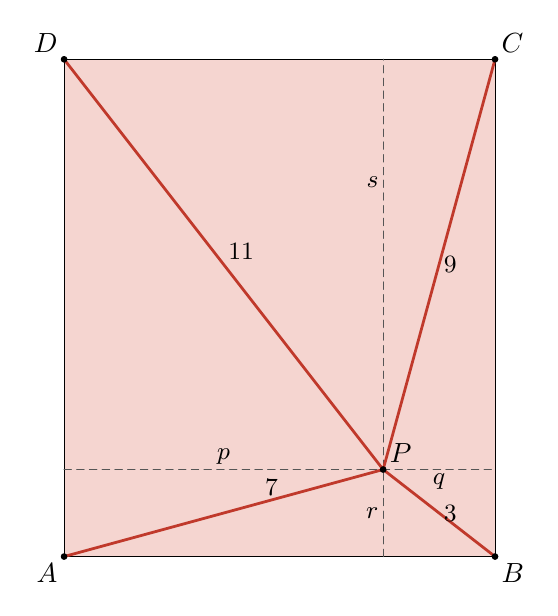
\begin{tikzpicture}
\tkzDefPoint(0.0,0.0){A} %! A = (0, 0)
\tkzDefPoint(5.4728420,0.0){B} %! B = (104/k, 0)
\tkzDefPoint(5.4728420,6.3148177){C} %! C = (104/k, 120/k)
\tkzDefPoint(0.0,6.3148177){D} %! D = (0, 120/k)
\tkzDefPoint(4.0520080,1.1050931){P} %! P = (77/k, 21/k)
\tkzDefPoint(0.0,1.1050931){Fp} %! Fp = (0, 21/k)
\tkzDefPoint(5.4728420,1.1050931){Fq} %! Fq = (104/k, 21/k)
\tkzDefPoint(4.0520080,0.0){Fr} %! Fr = (77/k, 0)
\tkzDefPoint(4.0520080,6.3148177){Fs} %! Fs = (77/k, 120/k)
%! fact dist(P, A) == 7
%! fact dist(P, B) == 3
%! fact dist(P, C) == 9
%! fact dist(P, D) == 11
%! fact area(A, B, C, D) == 96
%! fact perp(A, B, B, C)
%! fact perp(B, C, C, D)
%! fact perp(C, D, D, A)
%! fact perp(P, Fp, D, A)
%! fact perp(P, Fr, A, B)
%! fact collinear(Fp, P, Fq)
%! fact collinear(Fr, P, Fs)
%! fact dist(P, Fp) * dist(P, Fq) == dist(P, Fr) * dist(P, Fs)
%! fact dist(P, A) * dist(P, C) + dist(P, B) * dist(P, D) == 96
\tkzFillPolygon[color=figaccenttint](A,B,C,D)
\tkzDrawPolygon(A,B,C,D)
\tkzDrawSegments[aux](Fp,Fq Fr,Fs)
\tkzDrawSegments[key](P,A P,B P,C P,D)
\tkzDrawPoints(A,B,C,D,P)
\tkzLabelPoint[below left,lbl](A){$A$}
\tkzLabelPoint[below right,lbl](B){$B$}
\tkzLabelPoint[above right,lbl](C){$C$}
\tkzLabelPoint[above left,lbl](D){$D$}
\tkzLabelPoint[above right,lbl](P){$P$}
\tkzLabelSegment[above,pos=.35,len](P,A){$7$}
\tkzLabelSegment[right,pos=.5,len](P,B){$3$}
\tkzLabelSegment[right,pos=.5,len](P,C){$9$}
\tkzLabelSegment[above right,pos=.5,len](P,D){$11$}
\tkzLabelSegment[above,pos=.5,len](Fp,P){$p$}
\tkzLabelSegment[below,pos=.5,len](P,Fq){$q$}
\tkzLabelSegment[left,pos=.5,len](P,Fr){$r$}
\tkzLabelSegment[left,pos=.7,len](P,Fs){$s$}
\end{tikzpicture}
\end{document}
